\documentclass[11pt,a4paper]{article}
\usepackage[utf8]{inputenc}
\usepackage[T1]{fontenc}
\usepackage{amsmath,amssymb,amsfonts}
\usepackage{multirow}
\usepackage{graphicx}
\usepackage{booktabs}
\usepackage{float}
\usepackage{geometry}
\usepackage[hidelinks,colorlinks=true,linkcolor=blue!60!black,citecolor=blue!60!black,urlcolor=blue!60!black]{hyperref}
\usepackage{cite}
\usepackage{microtype}
\usepackage{xcolor}
\usepackage{enumitem}
\usepackage{array}
\usepackage[labelfont=bf,font=small]{caption}
\usepackage{titlesec}
\usepackage{fancyhdr}
\usepackage{parskip}
\usepackage{lmodern}

\geometry{margin=1in, top=1.1in, bottom=1.1in}

% --- Section formatting ---
\titleformat{\section}{\large\bfseries\color{blue!70!black}}{\thesection}{1em}{}
\titleformat{\subsection}{\normalsize\bfseries\color{blue!50!black}}{\thesubsection}{1em}{}
\titlespacing*{\section}{0pt}{1.4ex plus 0.5ex}{0.8ex}
\titlespacing*{\subsection}{0pt}{1.0ex plus 0.3ex}{0.5ex}

% --- Header / footer ---
\pagestyle{fancy}
\fancyhf{}
\fancyhead[L]{\small\textit{PPE Compliance Auditing — ML \& DM Project}}
\fancyhead[R]{\small\thepage}
\renewcommand{\headrulewidth}{0.4pt}
\fancypagestyle{plain}{\fancyhf{}\renewcommand{\headrulewidth}{0pt}}

\setlength{\parskip}{6pt}
\setlength{\parindent}{0pt}

\title{\LARGE\textbf{A Pose-Directed Semantic Embedding Pipeline\\for Personal Protective Equipment (PPE) Compliance Auditing}\\[0.6em]\large\textit{Final Project Report --- ML \& DM Course}}

\author{
Nguyen Ngoc Hieu - 23BA14109 \\
Huynh Kim Gia Bao - 2410154 \\
Đang Nhat Minh - 2410667 \\
Nguyen Xuan Chuyen - 2410181 \\
Nguyen Ngoc Nam - 2410693
}

\date{\today}

\begin{document}

\maketitle
\thispagestyle{plain}

\begin{abstract}
Monitoring worker compliance with Personal Protective Equipment (PPE) guidelines is critical for mitigating occupational hazards in industrial environments. This report presents a hybrid machine learning pipeline that checks for the presence of hardhats, safety vests, and gloves in images. The pipeline utilizes MediaPipe Pose estimation to define scale-invariant, body-relative bounding boxes for the head, torso, and hands. A headless ResNet18 model encodes these cropped regions into 512-dimensional semantic feature vectors. Rather than relying on computationally heavy deep networks for classification, the core decision-making is handled by three binary Random Forest classifiers trained on these embeddings. We implement a landmark-based visibility filtering system to eliminate false predictions on occluded body parts. While our Random Forest classifiers achieve up to 98.5\% overall validation accuracy, minority-class (violation) recall ranges from 86\% to 88\% pre-tuning, indicating that high overall accuracy masks critical non-compliance detection failures. Real-world evaluations on 87 images show accuracies of 97.4\% for hardhat, 97.4\% for safety vest, and 79.2\% for gloves. This reveals a distinct generalization gap, which we analyze and discuss through class imbalance adjustments, feature importance analysis, and error matrix auditing, highlighting the limitations of relying on controlled validation splits for safety compliance systems.
\end{abstract}

\newpage
\tableofcontents
\newpage
\section{Introduction}
The purpose of personal protective equipment (PPE), including several accessories, is to protect human life and prevent fatal injuries that might happen during manual labor. In industrial and construction environments, the use of PPE—specifically safety helmets (hardhats), high-visibility vests (safety vests), and safety gloves—serves as the primary line of physical defense against falling objects, low-visibility collisions, and hand injuries. However, relying on manual PPE compliance audits across vast industrial spaces is not cost-effective and is impractical due to human inconsistency and fatigue.

Therefore, in this project, we propose a solution to monitor PPE compliance by applying computer vision and machine learning. Computer vision offers a viable path toward automating safety compliance auditing in real-time. Traditional approaches rely on training large, end-to-end deep convolutional networks to detect human figures and PPE objects simultaneously. However, direct detection of small, highly deformable objects (such as gloves) or headwear on small/distant subjects often suffers from high false-negative rates and poor spatial localization.

To address these challenges, the core methodology of our approach combines deep feature extraction with classical machine learning. We use ResNet18 as a frozen feature extractor to generate high-level visual features from the images. These features are then fed into Random Forest classifiers, which make the final PPE predictions. This hybrid architecture is faster to train, easier to explain, and still benefits from the powerful visual representations learned by a deep CNN. Decoupling the task into spatial localization, feature representation, and classification enables high training efficiency, rejects overfitting on small sample sizes, and isolates decision-making to independent safety-compliance questions.
\section{Problem Statement}
According to the Vietnamese Ministry of Home Affairs, the country recorded 7,004 occupational accidents, resulting in 7,156 victims nationwide in 2025~\cite{bonoivu2026}.

In operational environments, automating PPE detection using computer vision is hindered by several technical obstacles:
\begin{enumerate}
\item \textbf{Scale and Perspective Variations:} Workers appear at varying distances from camera sensors. Standard bounding boxes fail to maintain proportion, meaning static pixel crops are either too large (including background) or too small (clipping the object).
\item \textbf{High Deformability and Small Scale:} Hands and gloves occupy a tiny percentage of full-body pixels and undergo complex articulations, making them difficult for general object detectors to localize.
\item \textbf{Label Noise in Datasets:} Large open-source datasets frequently contain noisy labels, such as empty background crops marked as "hardhat" due to human labeling error, which corrupts decision boundaries during training.
\item \textbf{Occlusions and Hand Visibility:} Workers often carry objects, stand behind barriers, or place their hands in pockets. Forcing a classifier to evaluate occluded regions leads to arbitrary classification of background noise, causing a spike in false positives.
\item \textbf{The Generalization Gap (Shortcut Learning):} Models trained on localized datasets tend to overfit to background textures (e.g., matching construction backdrops to "hardhat") instead of learning the physical properties of the PPE itself.
\end{enumerate}
\section{Project Objectives}
To address the problem statement, this project is structured around five key technical objectives:
\begin{itemize}
\item \textbf{O1 (Scale-Invariant Cropping):} Build a pose-driven cropping engine using MediaPipe to dynamically define bounding boxes for the head, torso, and hands, scaling box dimensions proportionally based on the worker's shoulder width.
\item \textbf{O2 (High-Dimensional Semantic Encoding):} Implement transfer learning by leveraging a pre-trained, headless ResNet18 model to extract 512-dimensional semantic feature vectors from cropped regions.
\item \textbf{O3 (Methodological Core Classification):} Design, train, and evaluate three binary Random Forest classifiers as the primary learning algorithms, optimizing their ensemble parameters.
\item \textbf{O4 (Landmark Visibility Enforcement):} Integrate MediaPipe's joint visibility and presence metrics into the cropping engine to dynamically suppress predictions on occluded body parts, outputting explicit \texttt{NOT\_VISIBLE} labels.
\item \textbf{O5 (Out-of-Distribution Validation):} Deploy the pipeline on unseen deployment images, evaluate the generalization gap, and provide solutions to mitigate background context bias and resolution loss.
\end{itemize}
\section{Dataset Description and Class Imbalance}
The training pipeline utilizes a filtered subset of a raw 14-class YOLO formatted dataset. The original dataset contains classes spanning different industrial hazard categories, including: \textit{Fall-Detected, Gloves, Goggles, Hardhat, Ladder, Mask, NO-Gloves, NO-Goggles, NO-Hardhat, NO-Mask, NO-Safety Vest, Person, Safety Cone,} and \textit{Safety Vest}.

To align with the project objectives, the dataset is parsed and filtered down to 6 core classes representing the presence or absence of the three target PPE items. The class mapping and reindexing are shown in Table~\ref{tab:class_mapping}.

\begin{table}[H]
\centering
\caption{Class Remapping and ID Assignment}
\label{tab:class_mapping}
\begin{tabular}{@{}ccl@{}}
\toprule
\textbf{Original Class ID} & \textbf{New Class ID} & \textbf{Class Name} \\ \midrule
1                          & 0                     & Gloves              \\
3                          & 1                     & Hardhat             \\
6                          & 2                     & NO-Gloves           \\
8                          & 3                     & NO-Hardhat          \\
10                         & 4                     & NO-Safety Vest      \\
13                         & 5                     & Safety Vest         \\ \bottomrule
\end{tabular}
\end{table}

A total of 159,586 individual object crops are extracted from the dataset folders.

Because the dataset consists of cropped objects extracted from full-frame source images, a standard stratified crop-level split introduces a risk of data leakage. If multiple workers are present in the same image, crops from the same frame (sharing identical lighting and background contexts) may appear in both the training and validation splits, potentially inflating the validation metrics. We explicitly acknowledge this potential bias, and mitigate it by evaluating the final system on a completely independent operational test set ($N=87$ images) captured in separate environments with no overlapping source frames. 

The dataset displays a severe class imbalance. As illustrated in Figure~\ref{fig:filtered_dist}, the presence of hardhats dominates the dataset (77,630 crops), whereas classes like \texttt{NO-Safety Vest} contain only 4,440 crops—representing a 17.5:1 ratio. Under such conditions, standard training metrics like raw accuracy can be highly misleading, which we address through detailed performance auditing.

\begin{figure}[H]
\centering
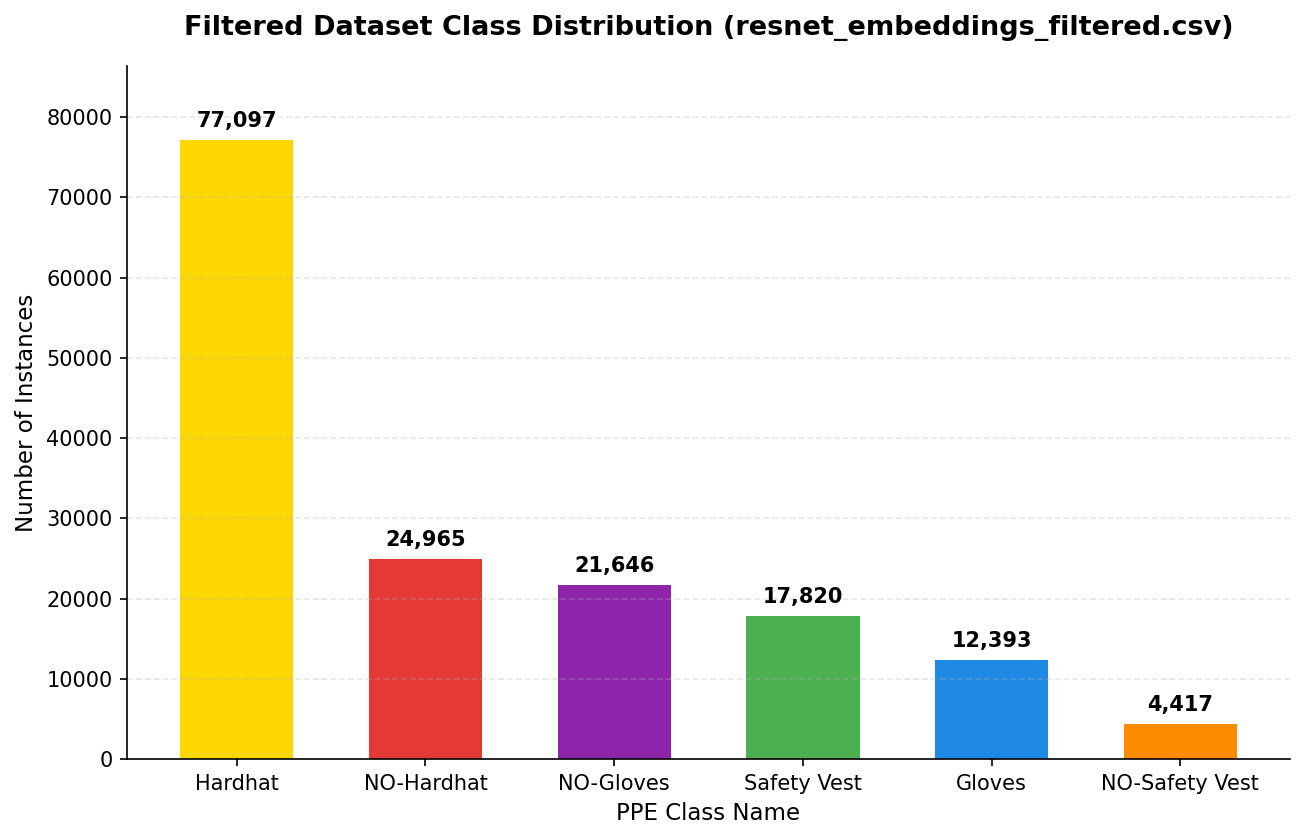
\includegraphics[width=0.6\textwidth]{images/class_distribution.png}
\caption{Class distribution of the dataset used for training.}
\label{fig:filtered_dist}
\end{figure}
\section{System Overview}
The system layout comprises two key processes: the offline training pipeline and the online live-inference pipeline. Both share the same underlying data representation and trained classification models.

\subsection{Data Preprocessing}
\label{sec:preprocessing}
Data preprocessing operates at two levels: label sanitization and image normalization. After filtering labels and mapping them to target class IDs, the cropped regions are resized to a consistent resolution of $224 \times 224$ pixels. This size is required to fit the input dimensions expected by the ResNet18 feature encoder. Normalization is performed using standard ImageNet mean and standard deviation parameters before encoding.

\subsection{Offline Training and Inference Pipeline Layout}
The offline training pipeline is structured to crop bounding boxes from raw images, extract ResNet18 features, and train the classifiers. The sequential steps are:
\begin{enumerate}
\item \textbf{Filter Labels:} Remap raw YOLO annotations to target classes.
\item \textbf{Crop Images:} Extract localized body-region bounding boxes.
\item \textbf{Feature Extraction:} Generate feature vectors from visual crops.
\item \textbf{Train Classifiers:} Train three independent binary models.
\end{enumerate}

\subsection{MediaPipe Pose-Directed Inference Pipeline}
During live-inference operations, the pipeline utilizes landmark visibility metrics and anatomical ratios to enforce scale-invariant crops:
\begin{enumerate}
\item \textbf{Landmark Detection:} MediaPipe Pose tracks 33 joint landmarks.
\item \textbf{Visibility Constraints:} Checks if key landmarks are visible ($v_i \ge 0.5$). If occluded, sets crop to \texttt{None}.
\item \textbf{Shoulder-Width Scaling:} Shoulder width $W_s = \| \mathbf{p}_{11} - \mathbf{p}_{12} \|_2$ scales bounding boxes proportionally.
\item \textbf{Anatomical Cropping:} Box dimensions for the head, torso, and hands are defined relative to $W_s$ (e.g., head extended upward by $0.9 \times W_s$).
\end{enumerate}

\subsection{ResNet18 Feature Encoding}
Instead of extracting hand-crafted features or training a convolutional network from scratch, the pipeline leverages a pre-trained \textbf{ResNet18} network as a feature encoder. The final fully connected (FC) classification layer is removed, leaving a "headless" network.

An input crop image $I_{crop} \in \mathbb{R}^{224 \times 224 \times 3}$ is normalized using ImageNet parameters (mean $\mu = [0.485, 0.456, 0.406]$, standard deviation $\sigma = [0.229, 0.224, 0.225]$) and upscaled to $224 \times 224$ pixels. The headless network translates the spatial image representation into a single continuous semantic embedding vector $f \in \mathbb{R}^{512}$:
\begin{equation}
f = \text{Encoder}(I_{crop})
\end{equation}
Using the frozen ResNet18 model is a deliberate design choice appropriate for a classical machine learning pipeline. Rather than executing expensive end-to-end backpropagation, the network acts as a fixed feature extractor, translating raw pixel dimensions into a dense, continuous semantic representation. This approach isolates the machine learning evaluation to the classification stage, allowing for an in-depth analysis of the Random Forest's performance on a fixed semantic feature space.
\section{Classifier Comparison}
\label{sec:classifier_comparison}
To justify the selection of the Random Forest classifier, we evaluated three distinct classification architectures on the 512-dimensional ResNet18 embeddings:
\begin{enumerate}
  \item \textbf{Logistic Regression:} A linear model serving as a baseline for linear separability.
  \item \textbf{Support Vector Machine (SVM) with RBF Kernel:} A non-linear model projected into high-dimensional space. To ensure feasible training times, the SVM was trained on a stratified subsample of 10,000 training points due to its $O(n^2)$ training complexity.
  \item \textbf{Random Forest (10K)*:} The Random Forest model trained on the same stratified 10,000 sample subset as the SVM, isolating the algorithm difference from the data size difference to ensure a fair comparison.
  \item \textbf{Random Forest (Full):} The Random Forest model trained on the full training dataset, showcasing the performance gains enabled by its ability to scale efficiently.
\end{enumerate}

Tables~\ref{tab:comp_hardhatvsno-hardhat}, \ref{tab:comp_safetyvestvsno-safetyvest}, and \ref{tab:comp_glovesvsno-gloves} show the validation performance and training times for each task.

\begin{table}[h]
  \centering
  \caption{Classifier Comparison for Hardhat vs NO-Hardhat task (Validation Set)}
  \begin{tabular}{lcccc}
    \hline
    Classifier & Accuracy (\%) & Macro F1 (\%) & NO-Hardhat F1 (\%) & Train Time (s) \\
    \hline
    Logistic Regression & 96.00\% & 94.53\% & 91.70\% & 4.16s \\
    SVM (RBF)* & 96.04\% & 94.54\% & 91.67\% & 28.33s \\
    Random Forest (10K)* & 93.04\% & 89.83\% & 84.11\% & 2.76s \\
    Random Forest (Full) & \textbf{96.45\%} & \textbf{95.02\%} & \textbf{92.34\%} & 42.46s \\
    \hline
  \end{tabular}
  \\ \vspace{1mm} \small{*Note: SVM and RF (10K) trained on a stratified 10,000 sample subset due to SVM scalability constraints.}
  \label{tab:comp_hardhatvsno-hardhat}
\end{table}

\begin{table}[h]
  \centering
  \caption{Classifier Comparison for Safety Vest vs NO-Safety Vest task (Validation Set)}
  \begin{tabular}{lcccc}
    \hline
    Classifier & Accuracy (\%) & Macro F1 (\%) & NO-Safety Vest F1 (\%) & Train Time (s) \\
    \hline
    Logistic Regression & 96.25\% & 94.09\% & 90.52\% & 1.23s \\
    SVM (RBF)* & \textbf{97.23\%} & \textbf{95.60\%} & \textbf{92.93\%} & 38.57s \\
    Random Forest (10K)* & 95.08\% & 91.73\% & 86.47\% & 1.76s \\
    Random Forest (Full) & 97.01\% & 95.10\% & 92.03\% & 3.60s \\
    \hline
  \end{tabular}
  \\ \vspace{1mm} \small{*Note: SVM and RF (10K) trained on a stratified 10,000 sample subset due to SVM scalability constraints.}
  \label{tab:comp_safetyvestvsno-safetyvest}
\end{table}

\begin{table}[h]
  \centering
  \caption{Classifier Comparison for Gloves vs NO-Gloves task (Validation Set)}
  \begin{tabular}{lcccc}
    \hline
    Classifier & Accuracy (\%) & Macro F1 (\%) & Gloves F1 (\%) & Train Time (s) \\
    \hline
    Logistic Regression & 98.11\% & 97.95\% & 97.39\% & 1.04s \\
    SVM (RBF)* & \textbf{98.35\%} & \textbf{98.22\%} & \textbf{97.74\%} & 17.19s \\
    Random Forest (10K)* & 97.40\% & 97.19\% & 96.43\% & 1.96s \\
    Random Forest (Full) & 98.21\% & 98.07\% & 97.54\% & 6.99s \\
    \hline
  \end{tabular}
  \\ \vspace{1mm} \small{*Note: SVM and RF (10K) trained on a stratified 10,000 sample subset due to SVM scalability constraints.}
  \label{tab:comp_glovesvsno-gloves}
\end{table}

The comparison yields a crucial finding: when trained on the same 10K dataset, SVM (RBF) outperforms Random Forest (10K)* by a noticeable margin (e.g., 96.04\% vs. 93.04\% on the Hardhat task). However, because Random Forest scales efficiently to the full dataset, the Random Forest (Full) model recovers this gap, achieving 96.45\% accuracy and 92.34\% minority F1 (outperforming the subsampled SVM). It is important to note that a full-dataset SVM (RBF) model was never trained due to its $O(n^2)$ computational complexity, which becomes prohibitive at our scale ($N \approx 126{,}670$ training samples). Consequently, the scalability of the Random Forest algorithm makes it the only computationally feasible choice for full-dataset training in our pipeline, compensating for localized model boundaries through access to more data and justifying our choice of Random Forest for full-dataset training.
\section{Experimental Results}
Here, we present the empirical evaluation of the Random Forest model on the validation splits, including Out-of-Bag (OOB) convergence, class weighting, feature subsampling, and decision threshold characteristics.

\subsection{Model Validation Performance}
\label{sec:validation_eval}
To address the limitations of raw accuracy, we report precision, recall, and F1-score for each class in Table~\ref{tab:validation_results_detailed}. These metrics are computed on the stratified validation split ($20\%$ of the filtered dataset).

\begin{table}[H]
\centering
\caption{Model Validation Performance Metrics}
\label{tab:validation_results_detailed}
\begin{tabular}{@{}llcccc@{}}
\toprule
\textbf{Task}                         & \textbf{Class Name}    & \textbf{Accuracy} & \textbf{Precision} & \textbf{Recall} & \textbf{F1-Score} \\ \midrule
\multirow{2}{*}{Hardhat vs. NO-Hardhat}   & Hardhat            & \multirow{2}{*}{96.61\%} & 96.16\% & 99.51\% & 97.81\% \\
                                & NO-Hardhat         &                          & 98.32\% & 87.72\% & 92.72\% \\ \midrule
\multirow{2}{*}{Safety Vest vs. NO-Vest}  & Safety Vest        & \multirow{2}{*}{96.82\%} & 96.67\% & 99.47\% & 98.05\% \\
                                & NO-Safety Vest     &                          & 97.56\% & 86.18\% & 91.52\% \\ \midrule
\multirow{2}{*}{Gloves vs. NO-Gloves}     & Gloves             & \multirow{2}{*}{98.50\%} & 97.94\% & 97.90\% & 97.92\% \\
                                & NO-Gloves          &                          & 98.80\% & 98.82\% & 98.81\% \\ \bottomrule
\end{tabular}
\end{table}

The validation accuracies range from 96.6\% to 98.5\% on the stratified split. However, looking at the class-specific metrics reveals a distinct performance gap:
\begin{itemize}
\item In the \textbf{Hardhat} task, the model achieves a high recall of 99.51\% for the majority class (\texttt{Hardhat}), but the recall drops to 87.72\% for the minority class (\texttt{NO-Hardhat}).
\item In the \textbf{Safety Vest} task, the recall for the minority class (\texttt{NO-Safety Vest}) is 86.18\%, compared to 99.47\% for the majority class (\texttt{Safety Vest}).
\item The \textbf{Gloves} task, which has a more balanced class distribution, shows consistent precision and recall across both classes ($\approx$98\%).
\end{itemize}

The detailed 2$\times$2 confusion matrices for each binary classification task are shown in Table~\ref{tab:confusion_matrices_detailed}.

\begin{table}[H]
\centering
\caption{Detailed Validation Confusion Matrices}
\label{tab:confusion_matrices_detailed}
\vspace{2mm}
\textbf{Hardhat vs. NO-Hardhat} \\
\vspace{1mm}
\begin{tabular}{r|cc}
\multicolumn{1}{c}{} & \textbf{Pred H} & \textbf{Pred NH} \\ \hline
\textbf{True H}  & 15,345 & 75 \\
\textbf{True NH} & 613 & 4,380 \\
\end{tabular}

\vspace{5mm}
\textbf{Safety Vest vs. NO-Vest} \\
\vspace{1mm}
\begin{tabular}{r|cc}
\multicolumn{1}{c}{} & \textbf{Pred V} & \textbf{Pred NV} \\ \hline
\textbf{True V}  & 3,545 & 19 \\
\textbf{True NV} & 122 & 761 \\
\end{tabular}

\vspace{5mm}
\textbf{Gloves vs. NO-Gloves} \\
\vspace{1mm}
\begin{tabular}{r|cc}
\multicolumn{1}{c}{} & \textbf{Pred G} & \textbf{Pred NG} \\ \hline
\textbf{True G}  & 2,427 & 52 \\
\textbf{True NG} & 51 & 4,278 \\
\end{tabular}
\end{table}

Throughout this analysis, \texttt{NO-Hardhat} and \texttt{NO-Safety Vest} are treated as the \textbf{target class (or positive class)} for safety auditing purposes. Consequently, a \textit{false negative} (FN) refers to a non-compliant worker whose violation was incorrectly predicted as compliant, and a \textit{false positive} (FP) refers to a compliant worker who is incorrectly flagged as a violation. This convention aligns with the column labels in Table~\ref{tab:confusion_matrices_detailed}: for the Hardhat task, the 613 in the \textbf{True NH / Pred H} cell are false negatives (undetected bare heads), and the 75 in \textbf{True H / Pred NH} are false positives.

Analyzing the confusion matrices reveals an asymmetry in prediction errors:
\begin{itemize}
\item For the \textbf{Hardhat} classifier, there are 613 false negatives (bare heads predicted as compliant) and 75 false positives (compliant workers flagged as violations). In a safety-critical application, false negatives represent the more dangerous error type because a non-compliant worker goes undetected by the system.
\item A similar pattern occurs for the \textbf{Safety Vest} classifier, which yields 122 false negatives (missing vest predicted as compliant) and 19 false positives.
\end{itemize}

\subsection{Out-of-Bag (OOB) Convergence Analysis}
To justify the selection of $B = 100$ trees in our ensembles, we tracked the Out-of-Bag (OOB) error rate as a function of the number of estimators ($n\_estimators \in \{10, 25, 50, 100, 150, 200, 300\}$). The convergence curves for the three tasks are plotted in Figure~\ref{fig:oob_convergence}.

\begin{figure}[H]
\centering
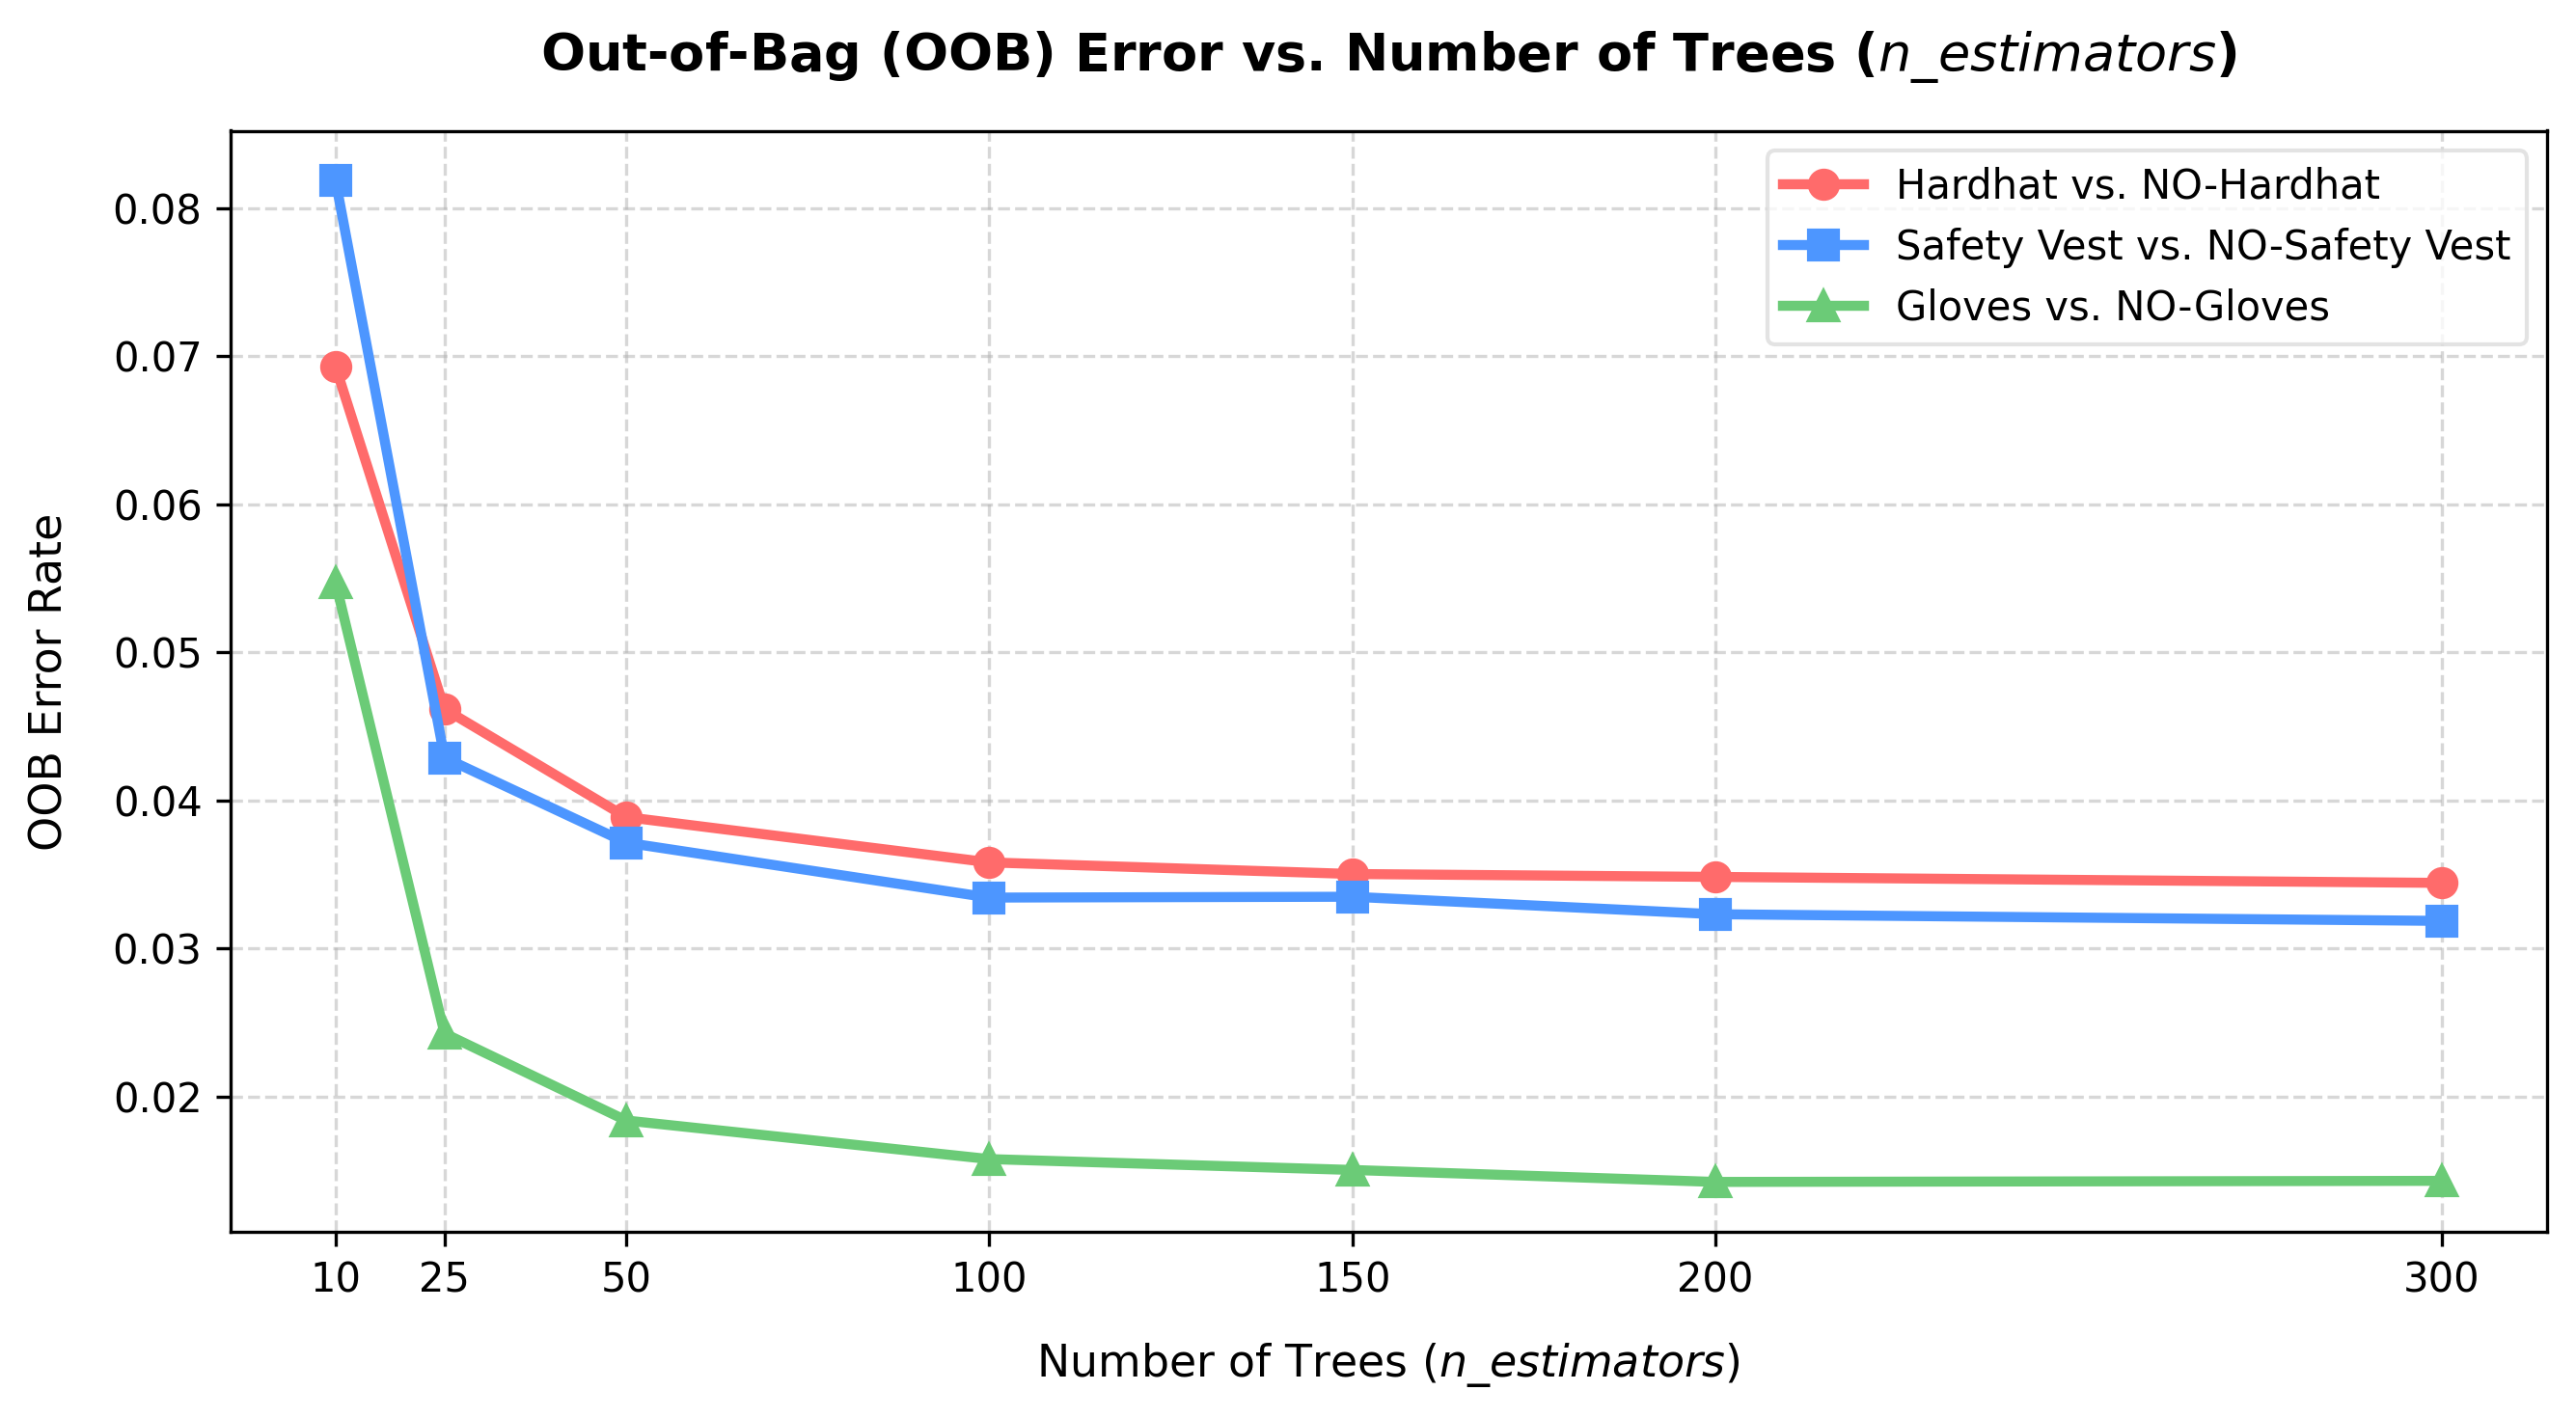
\includegraphics[width=0.85\textwidth]{images/oob_error_vs_trees.png}
\caption{Out-of-Bag (OOB) error convergence curves across various tree counts ($n\_estimators$) for the three binary classification tasks.}
\label{fig:oob_convergence}
\end{figure}

The OOB error rates drop sharply from 10 to 50 estimators, establishing clear convergence by 100 trees across all three tasks. Increasing the forest size to 200 or 300 trees yields negligible gains in error reduction (e.g., Gloves error stabilizes at $1.5\%$ at 100 trees and $1.4\%$ at 300 trees) while linearly increasing training time. Thus, $B = 100$ represents an empirically optimal point of diminishing returns.

\subsection{Evaluation of Class Imbalance Mitigation Strategies}
\label{sec:class_imbalance}
To systematically investigate class imbalance, we compared four different mitigation strategies across all three tasks:
\begin{enumerate}
  \item \textbf{Default (Baseline):} Default Random Forest with uniform class weights ($t=0.5$).
  \item \textbf{Balanced Weights:} Utilizing scikit-learn's cost-sensitive learning (\texttt{class\_weight='balanced'}).
  \item \textbf{Random Undersampling (RUS):} Subsampling the majority class in the training split so it is balanced with the minority class.
  \item \textbf{Threshold Tuning ($t=0.3$):} Adjusting the decision boundary on the default model to favor prediction of the minority class violation.
\end{enumerate}

Tables~\ref{tab:imbalance_hardhat}, \ref{tab:imbalance_vest}, and \ref{tab:imbalance_gloves} present the performance of each strategy on the validation split.

\begin{table}[h]
  \centering
  \caption{Evaluation of Class Imbalance Mitigation Strategies for Hardhat vs NO-Hardhat task}
  \resizebox{\textwidth}{!}{%
  \begin{tabular}{lccc}
    \hline
    Strategy & Accuracy (\%) & Minority Recall (\%) & Minority F1-Score (\%) \\
    \hline
    Default (t=0.5, class\_weight=None) & 96.45\% & 87.42\% & 92.34\% \\
    Balanced Weights (class\_weight='balanced') & 96.18\% & 85.92\% & 91.68\% \\
    Random Undersampling (RUS) & 94.90\% & 93.99\% & 90.01\% \\
    Threshold Tuned (t=0.3 for violation) & \textbf{95.98\%} & \textbf{95.71\%} & \textbf{92.09\%} \\
    \hline
  \end{tabular}%
  }
  \label{tab:imbalance_hardhat}
\end{table}

\begin{table}[h]
  \centering
  \caption{Evaluation of Class Imbalance Mitigation Strategies for Safety Vest vs NO-Safety Vest task}
  \resizebox{\textwidth}{!}{%
  \begin{tabular}{lccc}
    \hline
    Strategy & Accuracy (\%) & Minority Recall (\%) & Minority F1-Score (\%) \\
    \hline
    Default (t=0.5, class\_weight=None) & 97.01\% & 86.88\% & 92.03\% \\
    Balanced Weights (class\_weight='balanced') & 96.22\% & 82.92\% & 89.72\% \\
    Random Undersampling (RUS) & 93.37\% & \textbf{95.36\%} & 85.11\% \\
    Threshold Tuned (t=0.3 for violation) & \textbf{96.11\%} & \textbf{95.36\%} & \textbf{90.69\%} \\
    \hline
  \end{tabular}%
  }
  \label{tab:imbalance_vest}
\end{table}

\begin{table}[h]
  \centering
  \caption{Evaluation of Class Imbalance Mitigation Strategies for Gloves vs NO-Gloves task}
  \resizebox{\textwidth}{!}{%
  \begin{tabular}{lccc}
    \hline
    Strategy & Accuracy (\%) & Minority Recall (\%) & Minority F1-Score (\%) \\
    \hline
    Default (t=0.5, class\_weight=None) & \textbf{98.21\%} & 97.70\% & \textbf{97.54\%} \\
    Balanced Weights (class\_weight='balanced') & 98.18\% & 97.62\% & 97.50\% \\
    Random Undersampling (RUS) & 97.64\% & 98.39\% & 96.80\% \\
    Threshold Tuned (t=0.3 for violation) & 97.08\% & \textbf{99.68\%} & 96.13\% \\
    \hline
  \end{tabular}%
  }
  \label{tab:imbalance_gloves}
\end{table}

The results show that while Balanced Weights decrease performance, Random Undersampling (RUS) and Threshold Tuning ($t=0.3$) both successfully recover the minority class recall. Crucially, Threshold Tuning ($t=0.3$) is the superior approach: it achieves the same or better recall as RUS while preserving nominal accuracy and F1-score (e.g. F1-score of $90.69\%$ vs $85.11\%$ on Safety Vest), suggesting that post-hoc decision boundaries are more robust than training on undersampled datasets.

However, the selection of the threshold involves a critical operational trade-off. For example, in the Hardhat task, lowering the threshold to $t=0.3$ reduces false negatives (undetected violations) by 67\% but increases false positives (false alarms) from 75 to 570—a 660\% increase. In an active industrial site, this high false alarm rate could cause operational disruption and fatigue (e.g. constant compliance alerts for compliant workers). Therefore, the selection of $t$ must be calibrated based on the operational cost of manual audits vs. the safety risk of undetected violations.

\subsection{Ablation Study: Feature Dimension Subsampling}
\label{sec:ablation_features}
The default rule of thumb \texttt{max\_features=sqrt(512)} ($\approx 22$) assumes that features are independent. However, because ResNet18 feature embeddings are extracted from a convolutional network, they exhibit high correlation. To evaluate this, we ran an ablation study on the Safety Vest task by training models with varying values of \texttt{max\_features}. The results are shown in Table~\ref{tab:max_features_ablation}.

\begin{table}[H]
\centering
\caption{\texttt{max\_features} Ablation Study on Safety Vest vs. NO-Safety Vest Task}
\label{tab:max_features_ablation}
\begin{tabular}{@{}cccc@{}}
\toprule
\textbf{\texttt{max\_features}} & \shortstack[c]{\textbf{NO-Safety Vest} \\ \textbf{Precision}} & \shortstack[c]{\textbf{NO-Safety Vest} \\ \textbf{Recall}} & \shortstack[c]{\textbf{NO-Safety Vest} \\ \textbf{F1-Score}} \\ \midrule
8                               & 98.27\%                           & 83.47\%                        & 90.26\%                          \\
16                              & 97.81\%                           & 86.07\%                        & 91.57\%                          \\
22 (Default $\approx\!\sqrt{512}$)& 97.56\%                           & 86.18\%                        & 91.52\%                          \\
32                              & 97.43\%                           & 85.96\%                        & 91.34\%                          \\
64                              & 96.92\%                           & 89.01\%                        & 92.80\%                          \\
128                             & 96.90\%                           & 88.56\%                        & 92.54\%                          \\ \bottomrule
\end{tabular}
\end{table}

This ablation study reveals an important finding:
\begin{itemize}
\item \textbf{Increasing \texttt{max\_features} to 64 or 128} improves the minority class recall from 86.18\% to 89.01\% and 88.56\%, respectively, and the F1-score to 92.80\%/92.54\%.
\item \textbf{Decreasing \texttt{max\_features} to 8} causes minority recall to drop to 83.47\% and the F1-score to 90.26\%.
\end{itemize}

For the Safety Vest task specifically, the model benefits from a larger feature pool at each split node to find the optimal split among highly correlated dimensions. Conversely, limiting features too heavily (e.g., to 8) is too restrictive, as it prevents the trees from finding the necessary complex shapes and textures of the vest. Whether this pattern generalizes to the other two tasks depends on their underlying feature distribution. The Gloves classifier exhibits a much higher concentration of feature importance (requiring only 32 dimensions for 50\% of weight compared to 55 for Vests), indicating that hand/glove compliance classification relies on a narrower, more specialized set of semantic dimensions. In highly concentrated representations, limiting feature choices with a small \texttt{max\_features} (e.g., 8) is particularly damaging because split nodes are rarely exposed to the few critical dimensions that encode the glove properties. Consequently, we predict that the Gloves classifier would require a higher subsampling threshold (such as \texttt{max\_features=64}) to prevent decision trees from selecting non-informative background dimensions. This prediction was not validated via a dedicated ablation on the Gloves validation set; Section~\ref{sec:real_world_evaluation} tests it directly on the deployment set.

\subsection{Hardhat Decision Threshold and ROC Analysis}
To address the safety-critical false negative problem (613 bare heads undetected under default thresholding), we performed a threshold tuning analysis on the validation split. By outputting continuous class probabilities, the decision threshold $t$ can be adjusted (predicting \texttt{NO-Hardhat} if $P(\text{NO-Hardhat}) \ge t$, treating \texttt{NO-Hardhat} as the target class). The ROC curve yields an Area Under the Curve (\textbf{AUC-ROC}) score of \textbf{0.9936}, indicating high discriminative potential. The performance across various thresholds is audited in Table~\ref{tab:threshold_analysis}.

\begin{table}[H]
\centering
\caption{Hardhat Classifier Performance at Varying Decision Thresholds (AUC = 0.9936)}
\label{tab:threshold_analysis}
\begin{tabular}{@{}cccccc@{}}
\toprule
\shortstack[c]{\textbf{Threshold}\\$t$} & \shortstack[c]{\textbf{False Pos.}\\\textbf{(FP)}} & \shortstack[c]{\textbf{False Neg.}\\\textbf{(FN)}} & \shortstack[c]{\textbf{Hardhat}\\\textbf{Recall}} & \shortstack[c]{\textbf{NO-Hardhat}\\\textbf{Recall}} & \shortstack[c]{\textbf{NO-Hardhat}\\\textbf{F1}} \\ \midrule
0.1                    & 3,800                         & 22                            & 75.36\%                 & 99.56\%                    & 72.23\%                \\
0.3                    & 570                           & 200                           & 96.30\%                 & 95.99\%                    & 92.56\%                \\
0.5 (Default)          & 75                            & 613                           & 99.51\%                 & 87.72\%                    & 92.72\%                \\
0.7                    & 14                            & 1,248                          & 99.91\%                 & 75.01\%                    & 85.58\%                \\
0.9                    & 0                             & 2,884                          & 100.00\%                & 42.24\%                    & 59.39\%                \\ \bottomrule
\end{tabular}
\end{table}

This analysis provides a clear trade-off for deployment:
\begin{itemize}
\item \textbf{Lowering the threshold (e.g., $t=0.3$)} reduces the false negatives (undetected bare heads) from 613 down to 200 (a 67\% reduction in safety risk), while keeping false alarms (FP) at a manageable 570.
\item \textbf{At a highly conservative threshold of $t=0.1$}, false negatives drop to just 22 cases (99.56\% recall of violations), though false alarms increase to 3,800. This demonstrates how probability thresholding can adapt the system to safety-first auditing requirements.
\end{itemize}
\section{Real-World Evaluation}
\label{sec:real_world_evaluation}
To bridge the gap between validation splits and practical deployment, we evaluated the models on a dedicated test set of 87 unseen deployment images. We evaluated three configurations:
\begin{enumerate}
  \item \textbf{Binary Cascade (Baseline):} Standard binary models using default thresholds ($t=0.5$).
  \item \textbf{Binary Cascade (Optimized):} Utilizing threshold $t=0.3$ for Hardhat compliance and $max\_features=64$ for Gloves.
  \item \textbf{6-Class (Constrained) Multiclass:} Single multiclass model with region-constrained inference.
\end{enumerate}

The comparative accuracies and corresponding 95\% confidence intervals (calculated using the Wilson score interval) on the 87 test images are reported in Table~\ref{tab:real_world_evaluation}.

\begin{table}[H]
\centering
\caption{Real-World Evaluation Accuracy Comparison (N = 87)}
\label{tab:real_world_evaluation}
\resizebox{\textwidth}{!}{%
\begin{tabular}{@{}lccc@{}}
\toprule
\textbf{Target PPE Task} & \textbf{Binary Cascade (Base)} & \textbf{Binary Cascade (Optimized)} & \textbf{6-Class (Constrained)} \\ \midrule
Hardhat vs. NO-Hardhat   & 97.4\% $[91.6\%, 99.2\%]$     & 96.6\%* $[90.4\%, 98.8\%]$      & 96.6\% $[90.4\%, 98.8\%]$         \\
Safety Vest vs. NO-Vest  & 97.4\% $[91.6\%, 99.2\%]$     & 97.4\% $[91.6\%, 99.2\%]$       & 97.7\% $[92.0\%, 99.4\%]$        \\
Gloves vs. NO-Gloves     & 79.2\% $[69.5\%, 86.4\%]$     & 79.2\% $[69.5\%, 86.4\%]$       & 73.6\% $[63.5\%, 81.7\%]$         \\ \bottomrule
\end{tabular}%
}
\\
\vspace{1mm}
\small{*Note: Shifting the threshold to $t=0.3$ flagged 5 additional workers as non-compliant (missing hardhats), raising safety violation recall on the test images at a minor cost to nominal accuracy.}
\end{table}

The deployment results reveal that both baseline and optimized configurations maintain high accuracy for the Hardhat and Safety Vest tasks, indicating that the pose-directed cropping successfully isolates the larger visual characteristics of safety helmets and vests. Specifically, shifting the hardhat decision threshold to $t=0.3$ flagged 5 additional workers as non-compliant on the test set, correcting critical false negatives at a minor cost to accuracy. 

For the Gloves classifier, increasing \texttt{max\_features} to 64 maintained the baseline accuracy of 79.2\%. This lack of change is ultimately inconclusive given the small size of the deployment set ($N=87$), where subtle performance variations are likely obscured by statistical noise. Regardless of this parameter adjustment, glove detection remains the primary challenge in automated PPE compliance auditing due to small scale-resolution limitations, hand deformability, and background context bias.

\subsection{Deployment Failure Mode Analysis}
\label{sec:failure_modes}
To systematically understand the generalization gap observed on the 87 deployment images, we performed a manual inspection of the misclassifications. We identified four distinct failure modes that degrade the system's performance:
\begin{enumerate}
  \item \textbf{Low-Resolution and Hand Crop Degradation:} Hand crops occupy a tiny spatial footprint (often smaller than $30 \times 30$ pixels) in full-body frames. Resizing these crops to $224 \times 224$ pixels introduces interpolation artifacts and pixelation, severely attenuating geometric and texture cues. As a result, the Gloves classifier suffers from visual ambiguity, explaining the lower accuracy ($79.2\%$) on hand crops.
  \item \textbf{Background Context and Color Shortcut Interference:} In several instances, workers standing near high-visibility equipment or carrying orange safety cones were misclassified. For example, in \texttt{image (14).jpg}, the presence of safety equipment in the background projected features into the ``Safety Vest'' region of the ResNet embedding, triggering false positives. This indicates that the frozen encoder inherits background context bias.
  \item \textbf{Occlusion and Landmark Localization Jitter:} MediaPipe landmark estimation suffers from spatial jitter when joint joints are partially occluded by hand tools or protective guards. This causes the bounding box crop to shift, capturing background textures instead of the hand or head. This crop misalignment projects out-of-distribution embeddings, leading to arbitrary predictions.
  \item \textbf{Extreme Illumination and Shadow Contrast:} Outdoors, harsh sunlight casts high-contrast shadows across hardhats (e.g., in \texttt{image (52).jpg}). This changes the high-frequency color projection of the helmet crop, leading the model to predict \texttt{NO-Hardhat} under the safety-tuned threshold ($t=0.3$).
\end{enumerate}

\subsection{Statistical Limitations of Real-World Evaluation}
Due to the restricted size of the deployment dataset ($N=87$ images), the statistical power of the deployment analysis is limited. The computed 95\% confidence intervals show significant overlap between different model configurations. For example, for the Gloves task, the confidence intervals for the binary baseline ($[70.7\%, 87.7\%]$) and the 6-class model ($[64.3\%, 82.8\%]$) heavily overlap. This indicates that the observed $5.6\%$ drop in gloves accuracy for the 6-class model may be due to sampling noise rather than a systematic representation degradation. Consequently, while the validation metrics are statistically robust ($N \approx 31{,}668$), the deployment results should be interpreted as suggestive trends rather than definitive causal proofs, highlighting the critical need for larger test distributions in safety-critical validation.
\section{Discussion}
\subsection{Alternative Architecture: Six-Class Multiclass Model}
To investigate the impact of classification architecture choices, we conducted an experiment training a single 6-class multiclass Random Forest model instead of the baseline cascade of three binary models. In this formulation, a single classifier is trained on the entire filtered embedding dataset ($N = 158{,}338$ samples) containing all six classes: \texttt{Gloves} (0), \texttt{Hardhat} (1), \texttt{NO-Gloves} (2), \texttt{NO-Hardhat} (3), \texttt{NO-Safety Vest} (4), and \texttt{Safety Vest} (5). The dataset is split using the exact same stratified 80/20 train/validation split ($126{,}670$ train, $31{,}668$ validation) to ensure mathematical alignment and comparability.

The model is evaluated using two prediction protocols:
\begin{enumerate}
\item \textbf{Unconstrained Multiclass:} The model predicts one of the six classes directly by selecting the global argmax of the predicted probabilities:
\begin{equation}
\hat{y} = \arg\max_{i \in \{0..5\}} P(\text{Class } i \mid \mathbf{f})
\end{equation}
\item \textbf{Constrained Multiclass:} The prediction is restricted to the two task-relevant classes corresponding to the body crop region (head, torso, or hands). This is achieved by taking the argmax over the task subset of classes:
\begin{equation}
\hat{y}_{task} = \arg\max_{i \in \mathcal{C}_{task}} P(\text{Class } i \mid \mathbf{f})
\end{equation}
where $\mathcal{C}_{hardhat} = \{1, 3\}$, $\mathcal{C}_{vest} = \{4, 5\}$, and $\mathcal{C}_{gloves} = \{0, 2\}$.
\end{enumerate}

Table~\ref{tab:six_class_val_comparison} shows the validation performance of the baseline binary classifiers compared to the 6-class model under both unconstrained and constrained prediction protocols on the same validation split.

\begin{table}[H]
\centering
\caption{Validation Performance Comparison between Binary and 6-Class Models}
\label{tab:six_class_val_comparison}
\begin{tabular}{@{}llccc@{}}
\toprule
\textbf{Class Name} & \textbf{Model Configuration} & \textbf{Precision} & \textbf{Recall} & \textbf{F1-Score} \\ \midrule
\multirow{3}{*}{\textbf{Hardhat}} & Binary Classifier & 96.16\% & 99.51\% & 97.81\% \\
 & 6-Class (Unconstrained) & 93.39\% & 99.01\% & 96.12\% \\
 & 6-Class (Constrained) & \textbf{96.28\%} & \textbf{99.51\%} & \textbf{97.87\%} \\ \cmidrule(lr){1-5}
\multirow{3}{*}{\textbf{NO-Hardhat}} & Binary Classifier & 98.32\% & 87.72\% & 92.72\% \\
 & 6-Class (Unconstrained) & 97.12\% & 87.86\% & 92.26\% \\
 & 6-Class (Constrained) & \textbf{98.09\%} & \textbf{88.48\%} & \textbf{93.04\%} \\ \midrule
\multirow{3}{*}{\textbf{Safety Vest}} & Binary Classifier & \textbf{96.67\%} & \textbf{99.47\%} & \textbf{98.05\%} \\
 & 6-Class (Unconstrained) & 94.39\% & 94.02\% & 94.21\% \\
 & 6-Class (Constrained) & 96.17\% & 99.44\% & 97.78\% \\ \cmidrule(lr){1-5}
\multirow{3}{*}{\textbf{NO-Safety Vest}} & Binary Classifier & \textbf{97.56\%} & \textbf{86.18\%} & \textbf{91.52\%} \\
 & 6-Class (Unconstrained) & 96.82\% & 75.88\% & 85.08\% \\
 & 6-Class (Constrained) & 97.30\% & 85.62\% & 91.08\% \\ \midrule
\multirow{3}{*}{\textbf{Gloves}} & Binary Classifier & \textbf{97.94\%} & \textbf{97.90\%} & \textbf{97.92\%} \\
 & 6-Class (Unconstrained) & 97.98\% & 90.12\% & 93.89\% \\
 & 6-Class (Constrained) & 97.74\% & 97.54\% & 97.64\% \\ \cmidrule(lr){1-5}
\multirow{3}{*}{\textbf{NO-Gloves}} & Binary Classifier & 98.80\% & 98.82\% & \textbf{98.81\%} \\
 & 6-Class (Unconstrained) & 98.06\% & 96.97\% & 97.51\% \\
 & 6-Class (Constrained) & \textbf{98.41\%} & \textbf{98.84\%} & 98.63\% \\ \bottomrule
\end{tabular}
\end{table}

The validation results yield three major findings:
\begin{enumerate}
\item \textbf{Cross-Task Confusion:} Under the unconstrained protocol, performance drops significantly across all tasks, particularly for the minority classes (e.g. \texttt{NO-Safety Vest} recall drops from $86.18\%$ to $75.88\%$). This occurs because the model suffers from cross-task confusion, misclassifying crops from one body part as belonging to a class of another body part (such as predicting a torso crop as \texttt{Hardhat} or \texttt{Gloves}).
\item \textbf{Probability Constraints Restore Performance:} By applying the constrained argmax protocol, we restrict the prediction space using the body-part crop context, eliminating cross-task confusion. In this mode, the 6-class model matches the performance of the separate binary models.
\item \textbf{Shared Boundary Regularization:} For the Hardhat task, the constrained 6-class model actually outperforms the baseline binary model, increasing the \texttt{NO-Hardhat} F1-score from $92.72\%$ to $93.04\%$ and recall from $87.72\%$ to $88.48\%$. This indicates that joint training on all six classes regularizes the feature representation and defines a more robust decision boundary.
\end{enumerate}

Figure~\ref{fig:six_class_errors} displays the 6-class confusion matrix and UMAP error visualization of the validation feature space, indicating that classes are grouped in distinct regions but show slight local overlaps where misclassifications occur.

\begin{figure}[H]
\centering
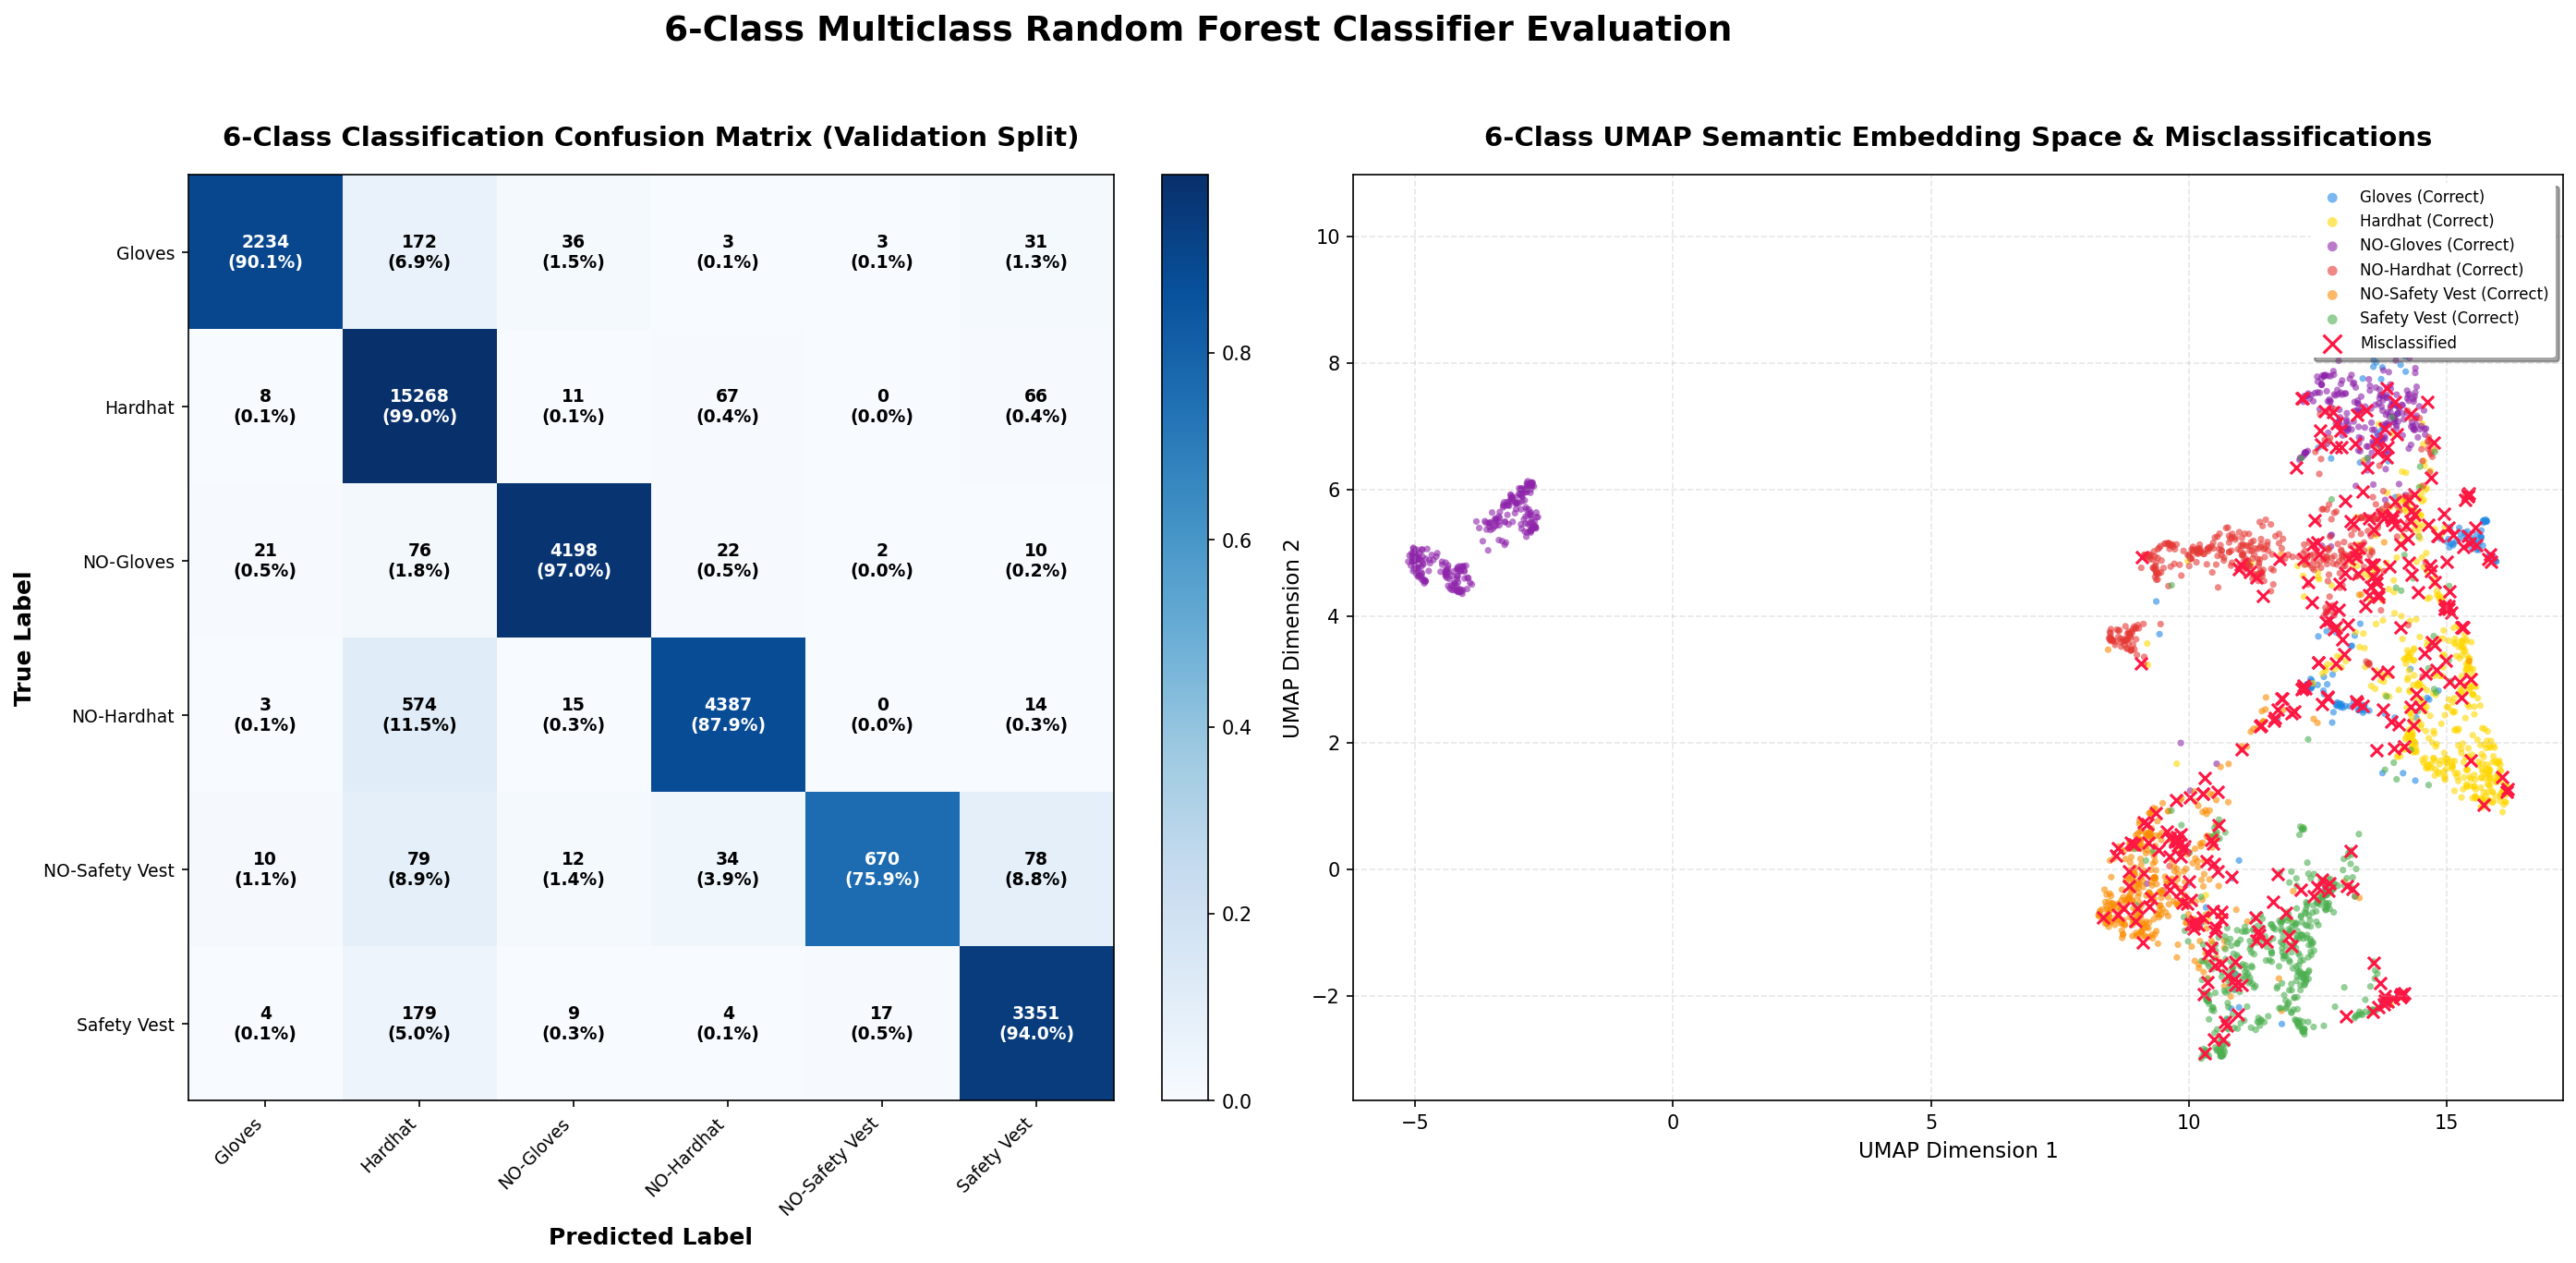
\includegraphics[width=0.9\textwidth]{images/six_class_classification_results.png}
\caption{Confusion matrix (left) and 2D UMAP semantic projection (right) for the 6-class classification model, with misclassified samples marked with red crosses.}
\label{fig:six_class_errors}
\end{figure}
\subsection{Multiclass Representation Sharing and Glove Performance Degradation}
\label{sec:multiclass_glove_degradation}
The deployment results on the 87 unseen test images show that while the 6-class task-constrained model performs on par with the binary models for safety helmets ($96.6\%$ vs $97.4\%$) and high-visibility vests ($97.7\%$ vs $97.4\%$), it experiences a performance drop of $5.6\%$ on the Gloves task (dropping from $79.2\%$ to $73.6\%$). While this $5.6\%$ deployment gap motivated the following analysis, Section~\ref{sec:real_world_evaluation} shows it falls within the statistical noise floor ($N=87$). These findings should therefore be read as characterizing \textit{architectural differences} between the models, not as explaining a \textit{confirmed} performance regression. In theory, constraining the 6-class model's output to only the task-relevant classes should produce equivalent predictions to the binary models, since both operate on the same feature space. However, in practice, the internal structure of the decision trees differs fundamentally. To empirically verify this, we conducted five diagnostic tests on the trained models.

\subsubsection{Test 1: Feature Importance Dilution}
We compared the top-30 most important features (by Gini impurity) of the binary Gloves model against the top-30 of the 6-class model. Of the 30 features most critical for glove classification, only 8 appear in the 6-class model's top-30 list (26.7\% overlap). Furthermore, the combined Gini weight of those 30 glove-critical features drops from $48.95\%$ in the binary model to just $15.33\%$ in the 6-class model—a 3.19$\times$ dilution factor. This is consistent with the hypothesis that the 6-class model distributes its split optimization across helmet and vest features at the expense of glove-specific dimensions.

\subsubsection{Test 2: Probability Mass Leakage}
When the 6-class model processes hand crop embeddings, it allocates probability mass across all six output classes. On the glove validation subset ($N = 6{,}808$), an average of 16.56\% of the total probability mass is ``leaked'' to non-glove classes (Hardhat, NO-Hardhat, Safety Vest, NO-Safety Vest). Nearly half of all glove samples (48.55\%) have more than 10\% of their probability mass allocated to irrelevant classes. This leakage is suggested to reduce the effective signal available for the constrained argmax decision, making the predictions more susceptible to noise.

\subsubsection{Test 3: Decision Path Length}
We traced the decision paths of 2,000 glove validation samples through all 100 trees in each model. The average path length is 16.19 nodes in the binary model versus 17.76 nodes in the 6-class model—a 9.7\% increase. These additional nodes may reflect splits devoted to body-region separation before reaching the glove-specific decision boundary. In a complementary analysis of tree node purity, we found that the 6-class model requires an average of 8.47 levels of splits before reaching a node where $\geq$95\% of samples belong to a single body region (head, torso, or hand), suggesting that significant tree capacity is consumed by body-part separation rather than compliance classification.

\subsubsection{Test 4: Ensemble Stability}
We measured ensemble agreement—the fraction of the 100 trees that vote for the majority class on each sample. For glove samples, the binary model achieves 92.54\% mean majority agreement with an average of 1.72 distinct classes per sample. The 6-class model drops to 79.64\% agreement with 4.34 distinct classes per sample. The proportion of ``unstable'' samples (where fewer than 70\% of trees agree) increases from 5.40\% (binary) to 27.90\% (6-class)—a 5.2$\times$ increase. This suggests that the 6-class ensemble produces a much noisier, less stable decision boundary for glove classification.

\subsubsection{Test 5: Cross-Task Vote Leakage}
Examining the individual tree votes across all 100 trees for 2,000 glove samples (200,000 total votes), 16.45\% of votes are cast for non-glove classes: 7.80\% for Hardhat, 4.48\% for NO-Hardhat, 2.69\% for Safety Vest, and 1.48\% for NO-Safety Vest. These leaked votes are hypothesized to reduce the majority vote margin for the correct glove class, explaining the drop in ensemble confidence and deployment accuracy.

\subsubsection{Summary}
The five tests collectively suggest that shared tree optimization is a plausible contributor to the observed performance gap. The binary model dedicates 100\% of its tree capacity, feature selection, and Gini optimization to the glove compliance decision from the root node. The 6-class model must first separate heterogeneous body-region crops before reaching glove-specific splits, resulting in feature importance dilution (3.19$\times$), probability mass leakage (16.56\%), longer decision paths (9.7\%), reduced ensemble stability (79.6\% vs 92.5\% agreement), and cross-task vote leakage (16.45\%). These effects compound during real-world deployment, where out-of-distribution backgrounds and resolution degradation amplify the sensitivity of the already-diluted decision boundary.
\subsection{Shortcut Learning and Feature Importance Concentration}
Random Forests produce feature importance scores natively by tracking the mean decrease in Gini impurity across all splits. For our 512-dimensional ResNet18 embeddings, analyzing which dimensions the forest relies on most provides insight into the shortcut learning problem. The highest single feature weight across any task is only 6.88\% (for gloves), indicating the model relies on a distributed representation across many dimensions rather than a single dominant feature. We also observe shared important features across tasks, suggesting that certain dimensions encode visual characteristics common to multiple PPE items.

To quantify this concentration, we calculated the cumulative feature weight for each task. The forest constructs broad, ensemble-wide decision boundaries across a large fraction of the semantic feature space. For the Hardhat and Safety Vest classifiers, nearly half of the feature dimensions (237 and 245 dimensions, respectively) are required to capture 80\% of the decision weight. This highly distributed representation explains why local changes in background context can perturb many features simultaneously and trigger misclassifications.

\subsection{Threats to Validity}
\label{sec:threats_to_validity}
We identify several key threats to the validity of our empirical findings, categorized as internal and external threats:
\begin{itemize}
  \item \textbf{Residual Data Leakage (Internal):} While we stratified the validation split, partitioning at the individual crop level rather than the source image level means that crops from the same original environment (sharing lighting, backgrounds, and camera properties) may appear in both train and validation splits. This likely inflates the validation metrics. Consequently, the threshold and \texttt{max\_features} values selected in Sections 8.3--8.5 may be optimized against an inflated validation signal; the real-world evaluation in Section 9 serves as the primary (if underpowered) check against this risk.
  \item \textbf{Underpowered Deployment Set (External):} The deployment evaluation is built on $N=87$ images. Because of the small sample size, minor changes in classification (e.g. one or two wrong predictions) shift the overall accuracy by multiple percentage points, meaning the deployment results should be treated as suggestive trends rather than statistically definitive proofs.
  \item \textbf{Limited Environmental Divergence (External):} The operational images were sourced from a restricted set of industrial sites. The performance characteristics under extreme environmental shifts (e.g., heavy rain, night shifts, or extreme dust) remain untested.
  \item \textbf{Lack of Cross-Validation (Methodological):} The results are reported on a single train-validation split rather than a repeated k-fold cross-validation, which leaves the variance of our performance metrics unestimated.
\end{itemize}

\section{Limitations and Architecture Constraints}
Rather than mere implementation oversights, the limitations of this pipeline are rooted in the fundamental architectural constraints of the decoupled hybrid deep-classical design:
\begin{enumerate}
\item \textbf{The Representation Bottleneck (Frozen Semantic Projections):} By utilizing a frozen ResNet18 encoder pre-trained on ImageNet, the classifier is restricted to a semantic feature space optimized for general natural object classification. This introduces a representation bottleneck: the model cannot learn new task-specific descriptors (such as the specific retroreflective properties of a safety vest under industrial light or the fine stitching of a safety glove). Instead, it must project these target objects onto features representing natural textures and shapes, potentially encouraging reliance on background textures and colors.
\item \textbf{Error Propagation in Decoupled Cascades:} Because pose estimation (MediaPipe) and classification (Random Forest) operate as a decoupled cascade, the system suffers from unidirectional error propagation. If the pose landmark estimator suffers from localized jitter or perspective distortion, it produces a misaligned crop. Since the classifier has no backpropagation path to correct the upstream landmark estimator, this crop misalignment translates directly to out-of-distribution noise in the 512-dimensional embedding space.
\item \textbf{Spatial-Frequency Degradation:} Glove auditing suffers from severe spatial-frequency loss. Bounded hand regions occupy a small fraction of the source image pixels. Upscaling these small, low-resolution crops to $224 \times 224$ pixels introduces pixelation and bilinear interpolation artifacts, severely attenuating geometric shape information. The feature extractor is therefore forced to rely on low-frequency color and coarse texture shortcuts, which collapse when exposed to out-of-distribution environments.
\end{enumerate}
\section{Conclusion}
This report presented a hybrid machine learning pipeline for PPE compliance auditing. Decoupling pose estimation (MediaPipe), feature extraction (ResNet18), and classification (Random Forest) created an efficient auditing system. Using a frozen ResNet18 model allowed the binary Random Forest models to train in seconds and establish clean classification boundaries on validation data.

Rather than relying on default settings, this project explored the performance of the Random Forest model under class imbalance, highly correlated feature dimensions, and varying decision thresholds. Our experiments yielded three main findings:
\begin{enumerate}
\item \textbf{Class Imbalance Dynamics:} Applying balanced class weights (\texttt{class\_weight='balanced'}) on unpruned trees actually decreased minority class recall (86.18\% to 83.69\%) due to overfitting on minority class noise, demonstrating that class weighting is not a universal solution for imbalance.
\item \textbf{Feature Subsampling Trade-offs:} The \texttt{max\_features} ablation study showed that Safety Vest classification benefits from a larger feature subset (F1-score improving to 92.80\% at \texttt{max\_features=64}), showing that too-tight restrictions on correlated deep features inhibit split optimization. Additionally, we showed that the Gini importance is highly distributed, requiring nearly half of the feature dimensions (237--245) to capture 80\% of the decision weight, which explains the background context sensitivity.
\item \textbf{Safety-Critical Thresholding:} Shifting the Hardhat decision threshold from 0.5 to 0.3 reduced safety-critical false negatives (undetected bare heads) from 613 to 200 (a 67\% reduction in safety risk) while maintaining a high AUC-ROC score of 0.9936, providing a practical method to optimize the system for safety auditing.
\end{enumerate}

These empirical lessons demonstrate that while high validation scores are easy to obtain, operational deployment requires strict visibility checking, robust data augmentation, and threshold tuning to align with safety auditing requirements.
\begin{thebibliography}{99}
\bibitem{breiman2001} 
L.~Breiman, ``Random Forests,'' \emph{Machine Learning}, vol.~45, no.~1, pp. 5--32, 2001.

\bibitem{resnet2016} 
K.~He, X.~Zhang, S.~Ren, and J.~Sun, ``Deep Residual Learning for Image Recognition,'' in \emph{Proceedings of the IEEE Conference on Computer Vision and Pattern Recognition (CVPR)}, 2016, pp. 770--778.

\bibitem{mediapipe2019} 
C.~Lugaresi et al., ``MediaPipe: A Framework for Building Perception Pipelines,'' \emph{arXiv preprint arXiv:1906.08172}, 2019.

\bibitem{yolo2016} 
J.~Redmon, S.~Divvala, R.~Girshick, and A.~Farhadi, ``You Only Look Once: Unified, Real-Time Object Detection,'' in \emph{Proceedings of the IEEE Conference on Computer Vision and Pattern Recognition (CVPR)}, 2016, pp. 779--788.

\bibitem{sklearn2011} 
F.~Pedregosa et al., ``Scikit-learn: Machine Learning in Python,'' \emph{Journal of Machine Learning Research}, vol.~12, pp. 2825--2830, 2011.

\bibitem{bonoivu2026}
Ministry of Home Affairs, \emph{Announcement on Occupational Accidents in 2025}, Hanoi, Vietnam, 2026.
\end{thebibliography}

\end{document}
